\scanpage{8}

% ll. 1–5
\mspage{\textcircled{6}}
cqfd.

Ceci étant soient $p\ne q\in E(w)^*$ liés à $s,t$, on sait \inserted{donc} qu'ils sont non liés à $\zeta,\zeta',\eta,\eta'$ et non liés entre eux i.e. $E(w)^*=\{\zeta,\zeta',\eta,\eta',p,p',q,q'\}$, où $p'=\sigma p$, $q'=\sigma q$. On a $p$ non lié à $x$ (sinon $px$ appartiendrait à 2 triangles de sommets $s,t$)

% ll. 6–10
de $=$ $p$ non \unsure{lié|liée} à $y$, donc $p'$ lié à $x$ et $y$. de $=$ $q'$ lié à $x$ et $y$, i.e.
\[
\{p',q'\}=\widetilde\varphi_{wu}(\{x,y\})
\]
ce qui prouve le corollaire.

% left beside ll. 6–8
\figure{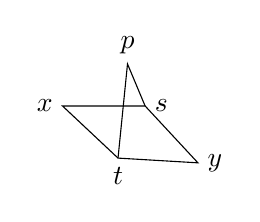
\begin{tikzpicture}[scale=.86]
\draw (0,0) node[left] {$x$} -- (1.22,0) node[right] {$s$} -- (2,-.84) node[right] {$y$} -- (.82,-.77) node[below] {$t$} -- cycle;
\draw (.82,-.77) -- (.96,.62) node[above] {$p$} -- (1.22,0);
\end{tikzpicture}}

% separator
\begin{center}\rule{2.2cm}{.35pt}\end{center}

% ll. 11–15
On identifie entre eux les $\Pi_{22}(P_u,P_v,P_w)$, soit $\unsure{J|\mathcal J|\sqsupset}$ de cardinal 3. [ Soit $V$ le \unsure{vectoriel|vectorl} de dim 2 sur $\mathbb F_2$ associé $(J=V^*)$ donc $P_u,P_v,P_w$ apparaissent comme des torseurs sous $V^*$. Soit $I=\{u,v,w\}$.

% ll. 16–18
\deleted{On a} Soit $\unsure{\widetilde{\mathscr T}|\widetilde\Gamma}$ l'ens des triangles $\subset S^*$, on voit que $\widetilde{\mathscr T}\xrightarrow{\sim}\prod_{\underbrace{x\in E(u)^*}_{\text{card. }8}}\underbrace{\unsure{w_v(u)|\omega_v(u)|\omega_v(x)}}_{\text{card }4}$ donc $\operatorname{Card}\widetilde{\mathscr T}=32$. Soit $\Gamma=\widetilde{\mathscr T}/\sigma$ (de cardinal 16)

% ll. 19–21
\uline{Lemme} 7 $\mathscr T\longrightarrow\underbrace{P_u\times P_v\times P_w}_{\text{cardinal }64=4.4.4}$ est : injectif, et \deleted{\unsure{$\mathscr T$}}\inserted{l'image de $\Gamma$} est un sous-torseur sous $\Psi(\unsure{W|V})\subset V\times V\times V$,

% l. 22
\[
(\Psi(V)=\{(x,y,z)\in V\times V\times V\mid x\unsure{+|-}y+z=0).
\]

% ll. 23–26
\uline{Dém} Soit $(x,s,\zeta),(y,t,\eta)$ deux triangles ayant $=$ image dans $P_u\times P_v\times P_w$. Quitte à appliquer $\sigma$ au $2^e$, \unsure{OPS|QPS} $y=x$. Alors $s$ et $t\in E(\unsure{u|v})^*$ liés à $x$ ne peut \deleted{être} satisfaire $t=\sigma s$, donc $t=s$, de $=$
% archive sheet number: 7
